\section{Eksperymenty}
W tym rozdziale opisane zostaną eksperymenty przeprowadzone w celu zbadania testów wydajnościowych środowisk uruchomieniowych. Testy zostały przeprowadzone na jednym komputerze wyposażonym w system operacyjny Linux, co pozwoliło na zminimalizowanie wpływu innych czynników na wyniki testów. 

\subsection{Algorytmy sortowania}
W celu zbadania wydajności danego środowiska uruchomieniowego, skonstruowana odpowiednie eksperymenty, które sprawdzają wydajność algorytmu sortowania. Wszystkie algorytmu sortowania zostały przetestowane dla każdego środowiska. W tabeli \ref{tab:sorting_experiments} przedstawiono ilość iteracji oraz ilość eksperymentów dla przeprowadzonych eksperymenty.

\begin{table}[H]
  \centering
  \begin{tabular}{|c|c|}
    \hline
    \textbf{Ilość iteracji} & \textbf{Ilość elementów} \\ \hline
    10 & 1000 \\ \hline
    100 & 1000 \\ \hline
    1000 & 1000 \\ \hline
    10 & 10000 \\ \hline
    100 & 10000 \\ \hline
    1000 & 10000 \\ \hline
  \end{tabular}
  \caption{Parametry eksperymentów}
  \label{tab:sorting_experiments}
\end{table}

\subsubsection{Wyniki}
W wykresach przedstawiono wyniki eksperymentów dla algorytmów sortowania bąbelkowego. Na osi X przedstawia liczbę iteracji, na osi Y czas wykonania algorytmu. 

\begin{figure}[h]
  \centering
  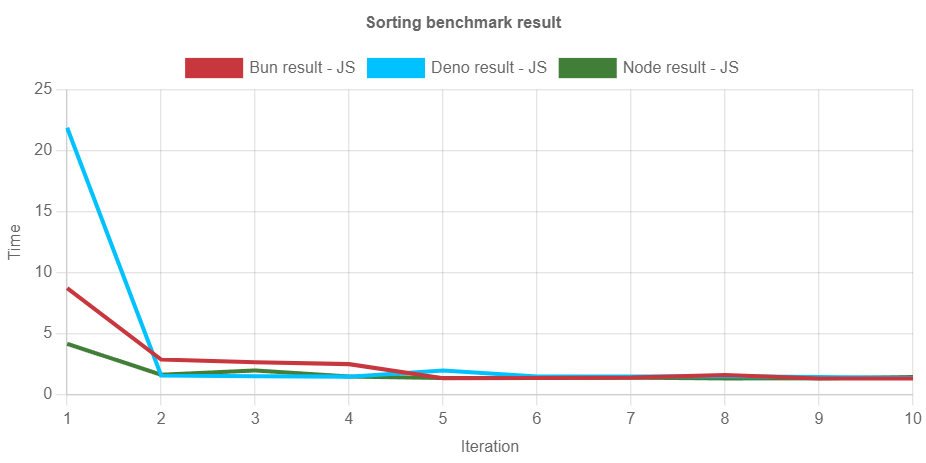
\includegraphics[width=0.7\textwidth]{Figures/sorting/bubble/e1_js.png}
  \caption{Wyniki eksperymentów dla algorytmu sortowania bąbelkowego}
  \label{fig:bubble_sorting_e1}
\end{figure}

Na wykresie \ref{fig:bubble_sorting_e1_memory} przedstawiono wyniki eksperymentów dla algorytmu sortowania bąbelkowego. Na osi X przedstawiono liczbę iteracji, natomiast na osi Y wykorzystanie pamięci. Jak widać, czas wykonania algorytmu rośnie wraz z ilością elementów.
\begin{figure}[h]
  \centering
  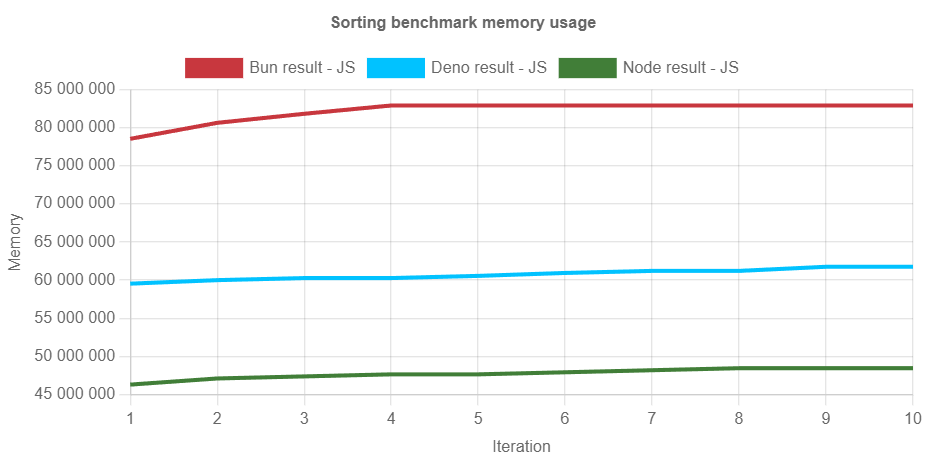
\includegraphics[width=0.7\textwidth]{Figures/sorting/bubble/e1_memory_js.png}
  \caption{Wyniki eksperymentów dla algorytmu sortowania bąbelkowego}
  \label{fig:bubble_sorting_e1_memory}
\end{figure}


\subsection{Algorytmy kodowania}

\subsubsection{Wyniki}

\subsection{Testy wydajnościowe operacji zapisu i odczytu plików}

\subsubsection{Wyniki}

\subsection{Testy wydajnościowe serwera HTTP}

\subsubsection{Wyniki}

\subsection{Testy wydajnościowe zapisu i odczytu danych z bazy danych}

\subsubsection{Wyniki}